\documentclass{beamer}


\usepackage{amsmath}
\usepackage{bookmark}
\usepackage{graphicx}
\usepackage{tikz-cd}
\usepackage{quiver}
\usepackage{mathtools}
\usepackage{bbm}


\usetheme{metropolis}

\mode<presentation>

%Information to be included in the title page:
\title{Modeling Open Systems \\with Category Theory}
\author{Daniel Sinderson}
\institute{Southern Oregon University}
\date{2024}

\begin{document}

\frame{\titlepage}

%\begin{frame}
%    \frametitle{Table of Contents}
%    \tableofcontents
%\end{frame}


%%%%%%%%%%%%%%%%%%%%%%%%%%%%%%%%%%%%%%%%%%%%%%%%%%%%%%%%%%%%%%%%%%%%%%%%%%%%%%%%%%%%%%%%%%%
%%%%%%%%%%%%%%%%%%%%%%%%%%%%%%%%%%%%%%%%%%%%%%%%%%%%%%%%%%%%%%%%%%%%%%%%%%%%%%%%%%%%%%%%%%%
\section{Objective and Scope of the Project}
%%%%%%%%%%%%%%%%%%%%%%%%%%%%%%%%%%%%%%%%%%%%%%%%%%%%%%%%%%%%%%%%%%%%%%%%%%%%%%%%%%%%%%%%%%%
%%%%%%%%%%%%%%%%%%%%%%%%%%%%%%%%%%%%%%%%%%%%%%%%%%%%%%%%%%%%%%%%%%%%%%%%%%%%%%%%%%%%%%%%%%%

\begin{frame}
    \frametitle{Goal of the Project}
    \begin{large}
        My objective for this project was to learn about the field of categorical systems theory,
        which applies the pure math field of category theory to the study of arbitrary systems,
        and then use what I learned to model a real-world system.
    \end{large}
\end{frame}

\begin{frame}
    \frametitle{The Scope of the Project}
    \begin{large}
        \begin{enumerate}
            \item Learn category theory
            \item Learn categorical systems theory
            \item Learn about a real world system
                  \\(transcription networks)
            \item Learn how to model and numerically solve it
                  \\(Julia language)
        \end{enumerate}
    \end{large}

\end{frame}

\begin{frame}
    \frametitle{Scope of this Presentation}
    \begin{large}
        \begin{enumerate}
            \item Tell you what a system is.
            \item Tell you what a category is.
            \item Tell you how they can work together.
            \item Show you a system and how I modeled it.
            \item Talk about the simulated results.
        \end{enumerate}
    \end{large}

\end{frame}



%%%%%%%%%%%%%%%%%%%%%%%%%%%%%%%%%%%%%%%%%%%%%%%%%%%%%%%%%%%%%%%%%%%%%%%%%%%%%%%%%%%%%%%%%%%
%%%%%%%%%%%%%%%%%%%%%%%%%%%%%%%%%%%%%%%%%%%%%%%%%%%%%%%%%%%%%%%%%%%%%%%%%%%%%%%%%%%%%%%%%%%
\section{Systems}
%%%%%%%%%%%%%%%%%%%%%%%%%%%%%%%%%%%%%%%%%%%%%%%%%%%%%%%%%%%%%%%%%%%%%%%%%%%%%%%%%%%%%%%%%%%
%%%%%%%%%%%%%%%%%%%%%%%%%%%%%%%%%%%%%%%%%%%%%%%%%%%%%%%%%%%%%%%%%%%%%%%%%%%%%%%%%%%%%%%%%%%


\begin{frame}{What is a System?}
    \begin{large}
        A system is a thing that changes. At its simplest, a system consists of the following two things.

        \begin{enumerate}
            \item A set of states that the system can be in.
            \item A map that updates the system's state based on the state that it's currently in.
        \end{enumerate}
    \end{large}


    \begin{center}
        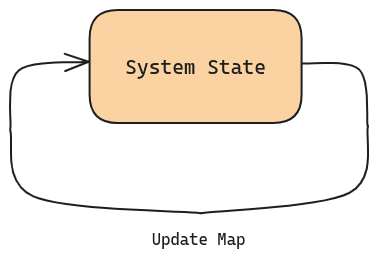
\includegraphics[scale=0.35]{system_diagram_closed.png}
    \end{center}

\end{frame}


\begin{frame}{Examples of Systems}
    \begin{large}
        The set of natural numbers with the successor function is a system.
        \vspace*{0.125in}
        \[
            S: \mathbb{N} \rightarrow \mathbb{N}
        \]
        \[
            \ \ \ \ \ \ \ \ \ n \mapsto n+1
        \]
    \end{large}
\end{frame}


\begin{frame}{Examples of Systems}
    \begin{large}
        An ordinary differential equation is also a system.
        \vspace*{0.125in}
        \[
            \frac{dx}{dt}=\kappa x
        \]
        Here the set of states is the set of real numbers $\mathbb{R}$ and the update map is the differential equation itself given some initial condition $x_0$.

    \end{large}

\end{frame}


\begin{frame}{What's the Problem}
    \begin{large}
        The problem with these systems is that they're closed.

        \vspace*{0.25in}
        They don't interact with each other, and they don't interact with their environment.

        \vspace*{0.25in}
        So let's open them up with category theory.
    \end{large}

\end{frame}







%%%%%%%%%%%%%%%%%%%%%%%%%%%%%%%%%%%%%%%%%%%%%%%%%%%%%%%%%%%%%%%%%%%%%%%%%%%%%%%%%%%%%%%%%%%
%%%%%%%%%%%%%%%%%%%%%%%%%%%%%%%%%%%%%%%%%%%%%%%%%%%%%%%%%%%%%%%%%%%%%%%%%%%%%%%%%%%%%%%%%%%
\section{Categories}
%%%%%%%%%%%%%%%%%%%%%%%%%%%%%%%%%%%%%%%%%%%%%%%%%%%%%%%%%%%%%%%%%%%%%%%%%%%%%%%%%%%%%%%%%%%
%%%%%%%%%%%%%%%%%%%%%%%%%%%%%%%%%%%%%%%%%%%%%%%%%%%%%%%%%%%%%%%%%%%%%%%%%%%%%%%%%%%%%%%%%%%

\begin{frame}{Category Theory Basics}
    \begin{large}
        Category theory is a theory of associative composition.

        \vspace*{0.25in}
        It's very general, and this generality allows it to encapsulate much of the high level structure in other theories.

        \vspace*{0.25in}
        This gives us a common formalism for working with the abstract structural features found across a multitude of diverse phenomena, both inside and outside of pure mathematics.

    \end{large}

\end{frame}


\begin{frame}{What is a Category?}
    \begin{definition}[Category]

        \vspace*{0.125in}
        A category $\mathcal{C}$ is defined by the following:
        \begin{enumerate}
            \item $\mathcal{C}$ contains a collection of objects $\mathsf{ob}(\mathcal{C})$.
            \item For any two objects $a$, $b$ $\in \mathcal{C}$ there is a collection of morphisms, $f:a \rightarrow b$, between those objects called the homset, $\mathcal{C}(a,b)$ .
            \item Every object $a\in \mathcal{C}$ has a morphism to itself $\mathsf{id}_a:a\rightarrow a$ called its identity.
            \item For every two morphisms $f:a\rightarrow b$ and $g: b\rightarrow c$ there's a third morphism $g\circ f:a\rightarrow c$ that's their composition.
        \end{enumerate}
    \end{definition}
\end{frame}



\begin{frame}[fragile]{What is a Category?}
    \begin{definition}[Category]
        \vspace*{0.125in}
        \[\begin{tikzcd}
                A && B && C \\
                \\
                && X
                \arrow["{\mathsf{id}_A}", from=1-1, to=1-1, loop, in=55, out=125, distance=10mm]
                \arrow["f", from=1-1, to=1-3]
                \arrow["{h \circ f}"', from=1-1, to=3-3]
                \arrow["{\mathsf{id}_B}", from=1-3, to=1-3, loop, in=55, out=125, distance=10mm]
                \arrow["h"', from=1-3, to=3-3]
                \arrow["g"', from=1-5, to=1-3]
                \arrow["{\mathsf{id}_C}", from=1-5, to=1-5, loop, in=55, out=125, distance=10mm]
                \arrow["{h \circ g}", from=1-5, to=3-3]
                \arrow["{\mathsf{id}_X}"', from=3-3, to=3-3, loop, in=305, out=235, distance=10mm]
            \end{tikzcd}\]
    \end{definition}
\end{frame}


\begin{frame}[fragile]{What is a Category?}
    These objects and morphisms are then under two constraints: unitality and associativity.
    \begin{definition}[Category cont. Unitality]
        Any morphism $f:a\rightarrow b$ can be composed with the identity morphisms of $a$ and $b$ such that $f\circ \mathsf{id}_a=\mathsf{id}_b\circ f=f$.
        \[\begin{tikzcd}
                a && b
                \arrow["{\mathsf{id}_a}"', from=1-1, to=1-1, loop, in=215, out=145, distance=10mm]
                \arrow["f", from=1-1, to=1-3]
                \arrow["{\mathsf{id}_b}", from=1-3, to=1-3, loop, in=325, out=35, distance=10mm]
            \end{tikzcd}\]
    \end{definition}
\end{frame}


\begin{frame}[fragile]{What is a Category?}
    These objects and morphisms are then under two constraints: unitality and associativity.
    \begin{definition}[Category cont. Associativity]
        For any morphisms $f:a\rightarrow b$, $g:b\rightarrow c$, and $h:c\rightarrow d$, $h\circ (g\circ f)=(h\circ g)\circ f$. Since it doesn't matter what order we apply the morphisms, we write this $h\circ g \circ f$.
        \[\begin{tikzcd}
                a & b & c & d
                \arrow["f"', from=1-1, to=1-2]
                \arrow["g"', from=1-2, to=1-3]
                \arrow["h"', from=1-3, to=1-4]
                \arrow["{{g\circ f}}", curve={height=-24pt}, from=1-1, to=1-3]
                \arrow["{{h\circ g}}"', curve={height=24pt}, from=1-2, to=1-4]
            \end{tikzcd}\]
    \end{definition}
\end{frame}




%%%%%%%%%%%%%%%%%%%%%%%%%%%%%%%%%%%%%%%%%%%%%%%%%%%%%%%%%%%%%%%%%%%%%%%%%%%%%%%%%%%%%%%%%%%%
%%%%%%%%%%%%%%%%%%%%%%%%%%%%%%%%%%%%%%%%%%%%%%%%%%%%%%%%%%%%%%%%%%%%%%%%%%%%%%%%%%%%%%%%%%%
\section{Composing Systems}
%%%%%%%%%%%%%%%%%%%%%%%%%%%%%%%%%%%%%%%%%%%%%%%%%%%%%%%%%%%%%%%%%%%%%%%%%%%%%%%%%%%%%%%%%%%
%%%%%%%%%%%%%%%%%%%%%%%%%%%%%%%%%%%%%%%%%%%%%%%%%%%%%%%%%%%%%%%%%%%%%%%%%%%%%%%%%%%%%%%%%%%
\begin{frame}{What is a Open System?}
    \begin{large}
        An open system is as a system with an interface.

    \end{large}

    \vspace*{0.25in}
    \begin{center}
        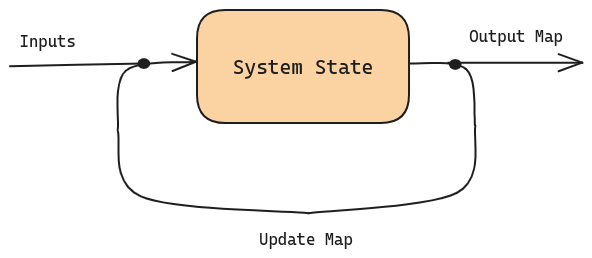
\includegraphics[scale=0.35]{system_diagram_open.png}
    \end{center}
\end{frame}


\begin{frame}{Lenses and Arenas}
    \begin{large}
        To model this mathematically we'll use objects called arenas and morphisms called lenses.

    \end{large}

    \vspace*{0.125in}
    \begin{definition}[Arenas]
        An arena is a pair of objects $\begin{pmatrix}A \\ B\end{pmatrix}$ from an underlying category.
    \end{definition}

    \begin{definition}[Lenses]
        \vspace*{0.125in}

        A lens is a morphism between arenas made from a pair of morphisms from the underlying category
        $$\begin{pmatrix}f \\ g\end{pmatrix}: \begin{pmatrix}A \\ B\end{pmatrix} \leftrightarrows \begin{pmatrix}C \\ D\end{pmatrix}$$
        where $g:B\rightarrow D$ is the output map and $f:B\times C \rightarrow A$ is the update map.
    \end{definition}
\end{frame}


\begin{frame}{What this Gives Us}
    \begin{large}
        Arenas and lenses between them form a monoidal category.

        \vspace*{0.125in}
        This means that we can compose systems and multiply them.

        \vspace*{0.125in}
        By modeling our open systems as lenses, composition of lenses lets us place systems in series and multiplication of lenses lets us place systems in parallel.

    \end{large}

\end{frame}


\begin{frame}{Systems in Series and Parallel}
    \begin{center}
        \begin{large}
            Systems in Series:
            $\begin{pmatrix}g^\# \\ g\end{pmatrix} \circ \begin{pmatrix}f^\# \\ f\end{pmatrix}$

            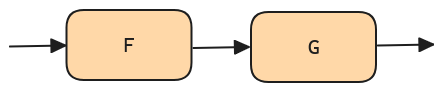
\includegraphics[scale=0.25]{Systems_Series.png}

            \vspace*{0.25in}
            Systems in Parallel:
            $\begin{pmatrix}g^\# \\ g\end{pmatrix} \otimes \begin{pmatrix}f^\# \\ f\end{pmatrix}$

            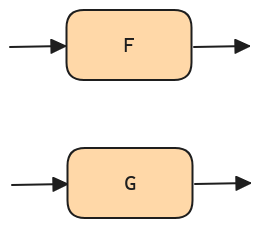
\includegraphics[scale=0.25]{Systems_Parallel.png}
        \end{large}
    \end{center}




\end{frame}

%%%%%%%%%%%%%%%%%%%%%%%%%%%%%%%%%%%%%%%%%%%%%%%%%%%%%%%%%%%%%%%%%%%%%%%%%%%%%%%%%%%%%%%%%%%
%%%%%%%%%%%%%%%%%%%%%%%%%%%%%%%%%%%%%%%%%%%%%%%%%%%%%%%%%%%%%%%%%%%%%%%%%%%%%%%%%%%%%%%%%%%
\section{Case Study}
%%%%%%%%%%%%%%%%%%%%%%%%%%%%%%%%%%%%%%%%%%%%%%%%%%%%%%%%%%%%%%%%%%%%%%%%%%%%%%%%%%%%%%%%%%%
%%%%%%%%%%%%%%%%%%%%%%%%%%%%%%%%%%%%%%%%%%%%%%%%%%%%%%%%%%%%%%%%%%%%%%%%%%%%%%%%%%%%%%%%%%%

\begin{frame}{Gene Transcription}
    \begin{large}
        Gene transcription is the process by which genes in a cell’s DNA produce proteins.

        \vspace*{0.125in}
        The dynamics of this process for a single gene are well modeled by the following differential equation.
        $$\frac{dY}{dt}=\beta f(X^*) - \alpha Y$$

        $$\text{Activator: } \ f_A(X^*)=\frac{\beta X^{*n}}{K^n + X^{*n}} \ \text{ or } \ \beta * L(X^* > K)$$
        $$\text{Repressor: } \ f_R(X^*)=\frac{\beta}{1 + \left(\frac{X^*}{K}\right)^n} \ \text{ or } \ \beta * L(X^* < K)$$

    \end{large}
\end{frame}

\begin{frame}{Motor Flagella Network}
    \begin{large}
        Gene transcription network are connected networks of genes whose products act as transcription factors for other genes.

        \vspace*{0.125in}
        Below is the motor flagella network of \textit{e. coli} bacteria.
    \end{large}


    \begin{center}
        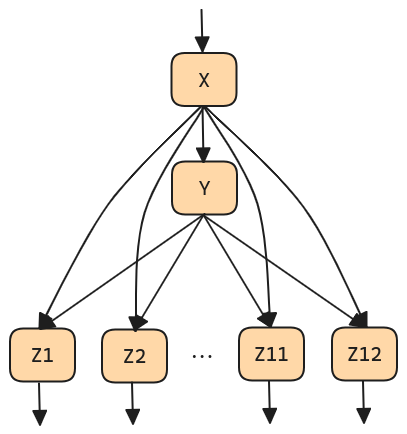
\includegraphics[scale=0.25]{multioutput_FFL_color.png}
        \hspace*{0.25in}
        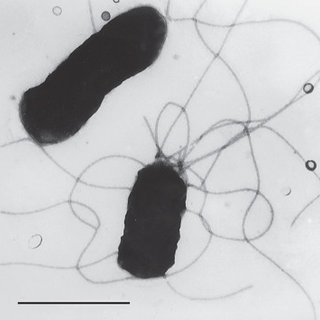
\includegraphics[scale=0.35]{Flagella-of-E-coli-observed-in-transmission-electron-microscope-Bar-1mm_Q320-2724765803.jpg}
    \end{center}

    \begin{footnotesize}
        \hspace*{\fill}Image from \textit{Bacterial Chemotaxis} by Michael Eisenbach
    \end{footnotesize}
\end{frame}


\begin{frame}{Motor Flagella Network Model}
    \begin{large}
        Using lenses we can wire together the transcription factor dynamics as differential systems and then simulate the results.

    \end{large}

    \begin{center}
        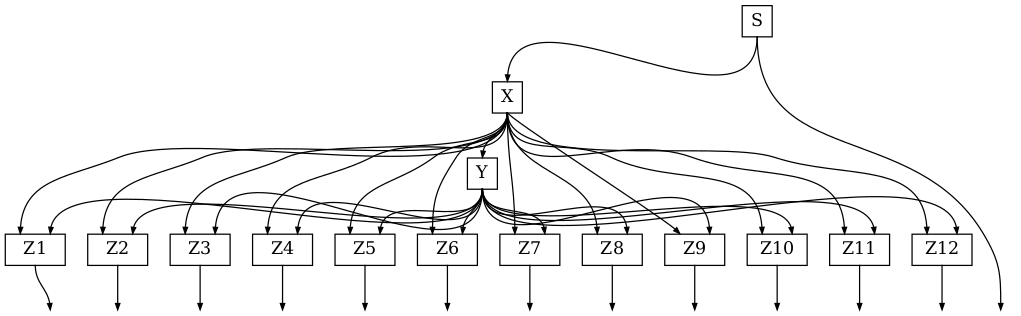
\includegraphics[scale=0.35]{motor_flagella_network.png}
    \end{center}

\end{frame}


\begin{frame}{Motor Flagella Network Model}
    %\begin{large}
    $$\text{Gene X: } \ \ \frac{dX}{dt} = [\beta*L(S > \kappa_S) - \alpha * X]$$
    $$\text{Gene Y: } \ \ \frac{dY}{dt} = [\beta*L(X > \kappa_X) - \alpha * Y]$$
    $$\text{Gene $Z1$: } \ \ \frac{dZ_1}{dt} = [\beta*L(X > \kappa_X \ \mathsf{OR} \ Y > \kappa_Y) - \alpha * Z_1]$$
    $$\text{Gene $Z2$: } \ \ \frac{dZ_2}{dt} = [\beta*L(X > \kappa_X \ \mathsf{OR} \ Y > \kappa_Y) - \alpha * Z_2]$$
    $$\vdots$$
    $$\text{Gene $Z11$: } \ \ \frac{dZ_{11}}{dt} = [\beta*L(X > \kappa_X \ \mathsf{OR} \ Y > \kappa_Y) - \alpha * Z_{11}]$$
    $$\text{Gene $Z12$: } \ \ \frac{dZ_{12}}{dt} = [\beta*L(X > \kappa_X \ \mathsf{OR} \ Y > \kappa_Y) - \alpha * Z_{12}]$$
    %\end{large}

\end{frame}



\begin{frame}{Motor Flagella Network Simulation Results}

    \begin{center}
        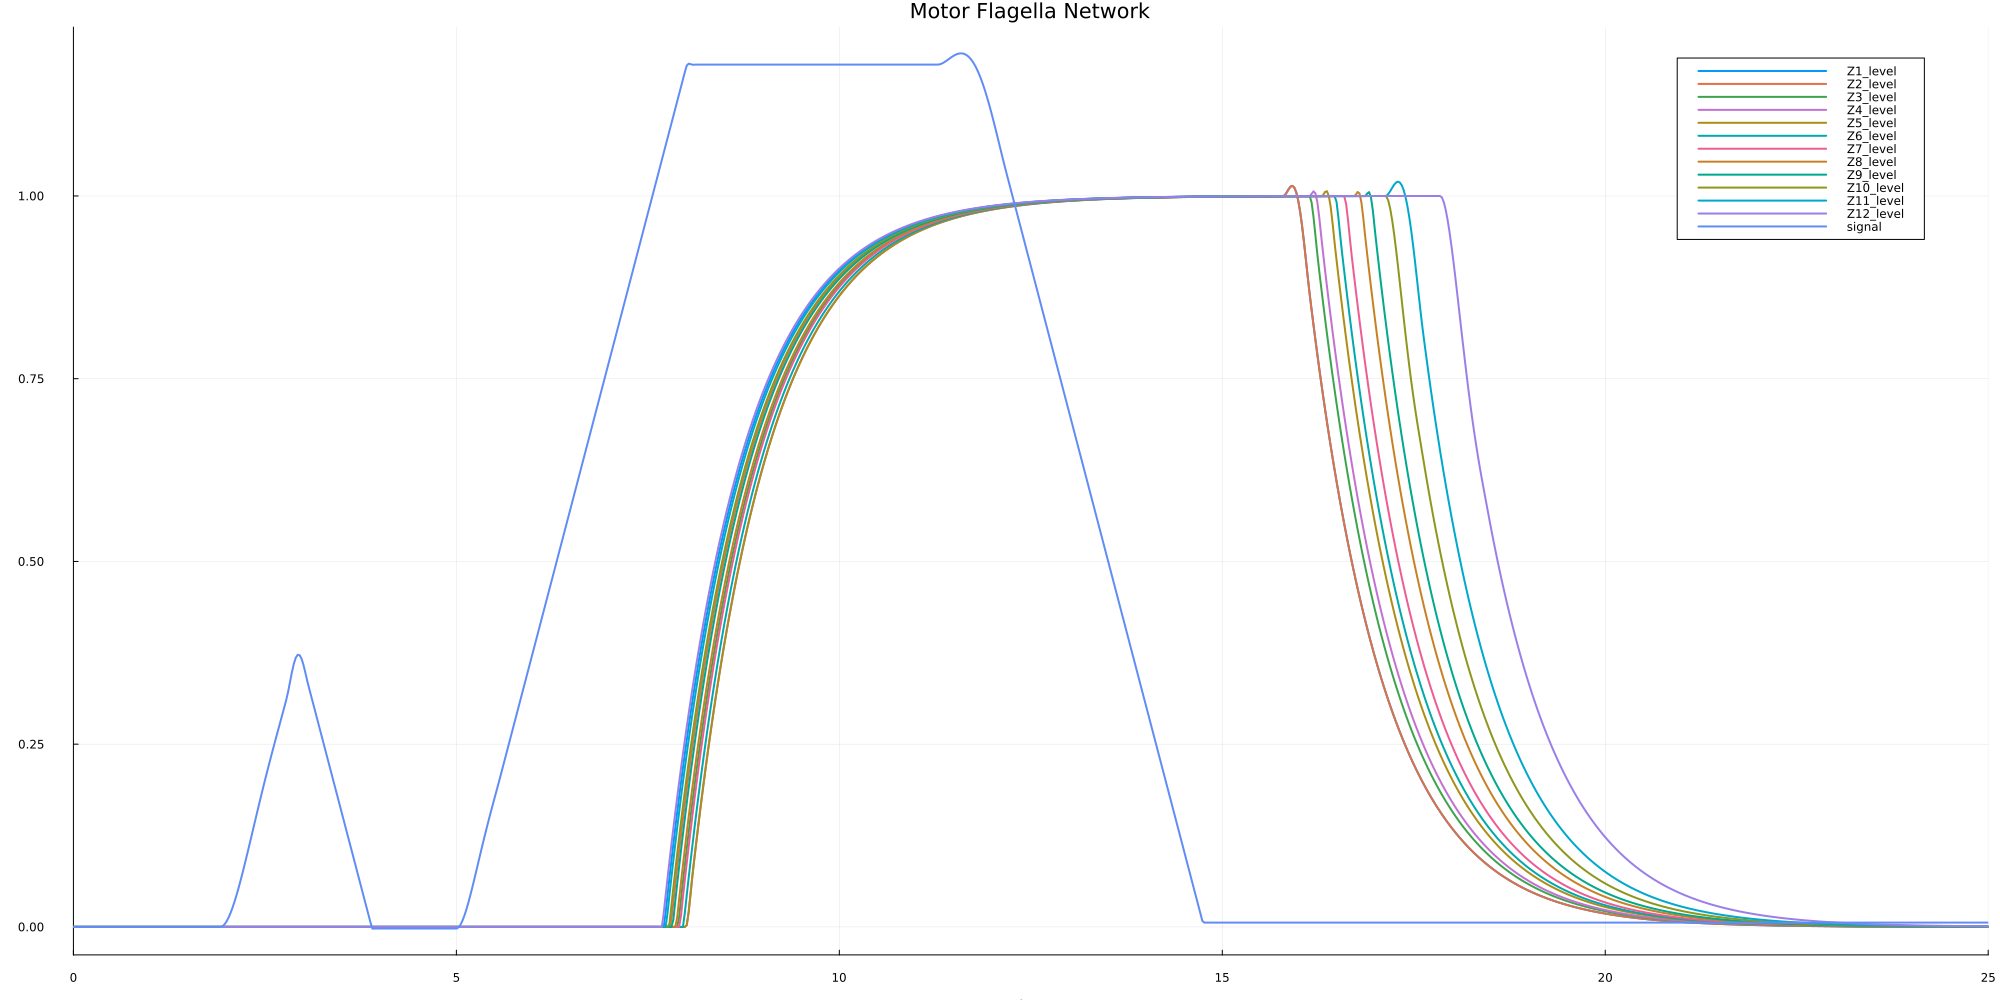
\includegraphics[scale=0.40]{motor_flagella.png}
    \end{center}

    \begin{footnotesize}
        Simulation results were obtained using the numerical solver in the OrdinaryDiffEq.jl library for the Julia programming language.
    \end{footnotesize}
\end{frame}


%%%%%%%%%%%%%%%%%%%%%%%%%%%%%%%%%%%%%%%%%%%%%%%%%%%%%%%%%%%%%%%%%%%%%%%%%%%%%%%%%%%%%%%%%%%
%%%%%%%%%%%%%%%%%%%%%%%%%%%%%%%%%%%%%%%%%%%%%%%%%%%%%%%%%%%%%%%%%%%%%%%%%%%%%%%%%%%%%%%%%%%
\section{Conclusion}
%%%%%%%%%%%%%%%%%%%%%%%%%%%%%%%%%%%%%%%%%%%%%%%%%%%%%%%%%%%%%%%%%%%%%%%%%%%%%%%%%%%%%%%%%%%
%%%%%%%%%%%%%%%%%%%%%%%%%%%%%%%%%%%%%%%%%%%%%%%%%%%%%%%%%%%%%%%%%%%%%%%%%%%%%%%%%%%%%%%%%%%


\begin{frame}{Where did all the Category Theory Go?}
    \begin{large}
        It's inside the wiring diagrams.

        \vspace*{0.25in}
        Diagrammatic languages are more intellectually tractable.

        \vspace*{0.25in}
        They are easier to reason about for both the designer or modeler and those they are designing or modeling for.

    \end{large}

\end{frame}


\begin{frame}{What's Next?}
    \begin{large}
        Lenses over other cartesian categories: $\textbf{Set}$, $\textbf{Man}$

        \vspace*{0.25in}
        Adding monads for nondeterministic systems: MDP, SDE

        \vspace*{0.25in}
        Using charts and double categories to compose system behavior as well as specification
    \end{large}

\end{frame}




\begin{frame}{}
    \begin{center}
        \begin{Huge}
            Thank You!
        \end{Huge}
    \end{center}
\end{frame}


\begin{frame}{References}
    \begin{thebibliography}{10}

        \bibitem{alon2019introduction}
        {\sc Alon, U.}
        \newblock {\em An introduction to systems biology: design principles of biological circuits}.
        \newblock Chapman and Hall/CRC, 2019.

        \bibitem{fong2019invitation}
        {\sc Fong, B., and Spivak, D.~I.}
        \newblock {\em An invitation to applied category theory: seven sketches in compositionality}.
        \newblock Cambridge University Press, 2019.

        \bibitem{myers2022categorical}
        {\sc Myers, D.~J.}
        \newblock Categorical systems theory.
        \newblock {\em Manuscript in preparation\/} (2022).
    \end{thebibliography}
\end{frame}



\end{document}